\subsection{Diseño de PCB}

Para el disenio del circuito en la placa se utilizó el programa KiCAD, se comenzo por su esquematico, tomando de referencia al brindado por la catedra

\begin{figure}[H]
  \centering
  \resizebox{250}{!}
  {
    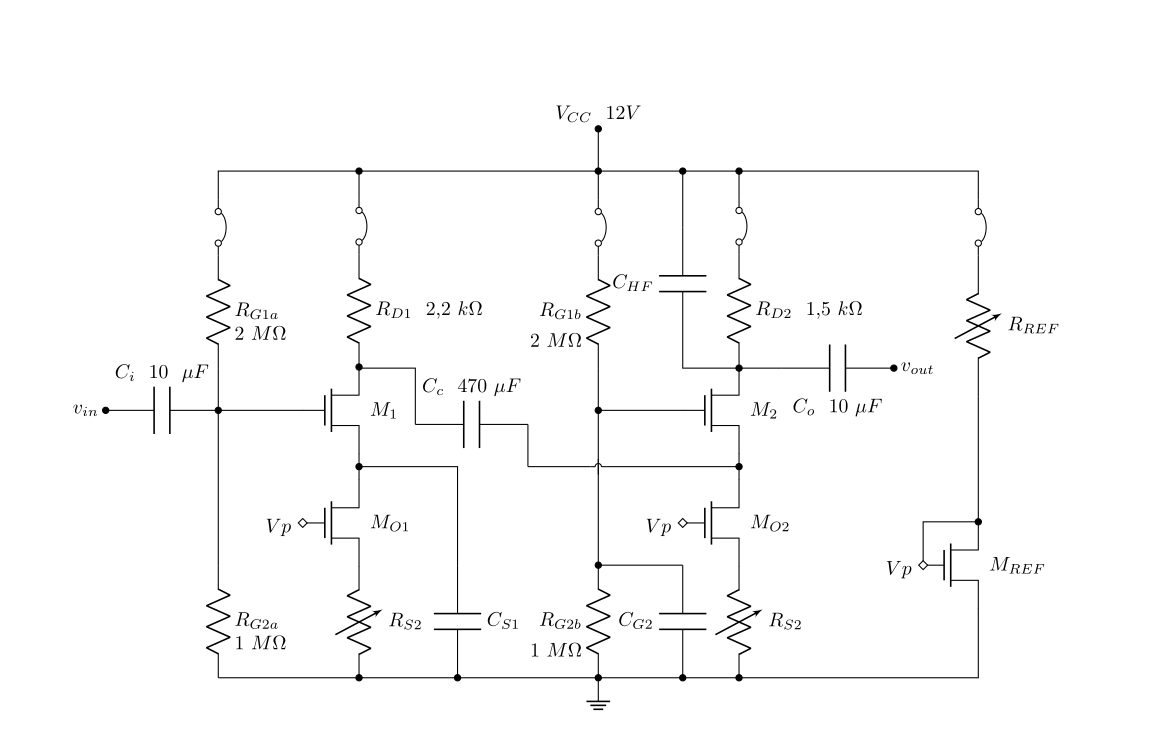
\includegraphics{Imagenes/EsquematicoCatedra.png}
  }
  \caption{Esquemático de la Catedra}
  \label{Esquematico_Cátedra}
\end{figure}

  Adicionalmente a este se le implementaron los siguientes componentes:
\begin{enumerate}
  \item Jumpers de aislación de etapas
  \item Test Points para la mediciones de Tension
  \item Headers macho a 90 grados para conectores BNC de entrada.
  \item Bornera doble de alimentación
  \item Jumpers de Aislacion de Presets
\end{enumerate}

Se tuvieron en cuenta las mediciones de la consigna para posicionar los puntos de prueba en el circuito, se optó por omitir aquellos Test Points en lugares donde los componentes de montaje brinden el espacio para su prueba con el fin de obtener un diseño más compacto y de menor costo.

\vspace{0.5em}
{\small\textbf{Diseño de Esquemático}}

Una vez constituido el esquemático (\ref{Esquematico}) a utilizar se le asignaron las huellas de los componentes, estas fueron designadas según la disipación de potencia estimada y las especifiaciones de MOSFET de la catedra.

\begin{figure}[H]
  \centering
  \resizebox{250}{!}{
    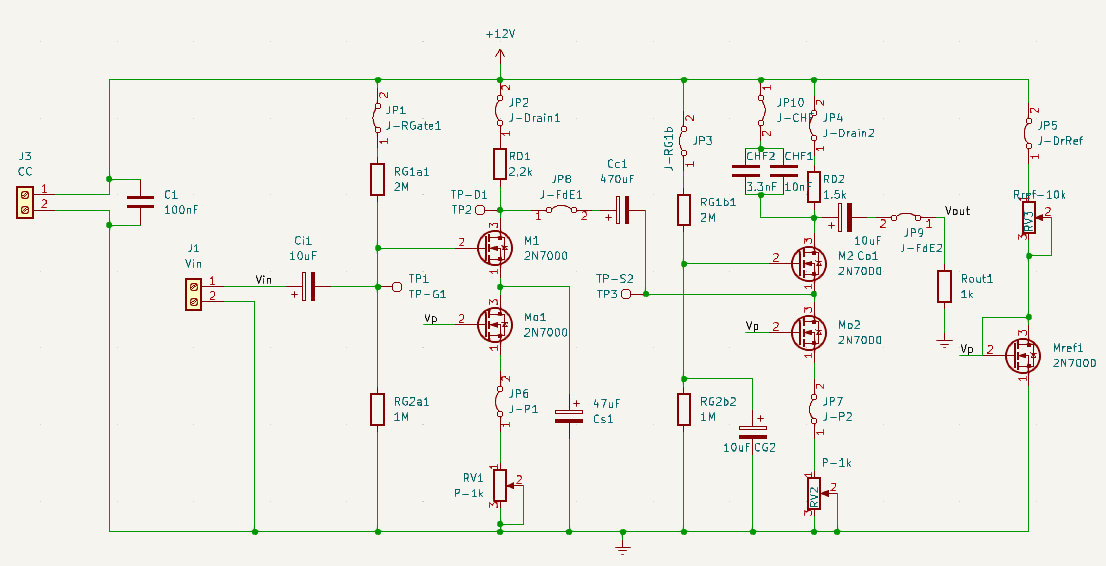
\includegraphics{Imagenes/Esquematico.png}
  }
  \caption{Esquemático del diseño final}
  \label{Esquematico}
\end{figure}

\vspace{0.5em}
{\small\textbf{Diseño de PCB }}

Para el enrutamiento (\ref{fig:trazas}) de los componentes y su disposición se tuvieron en cuenta diversos factores:

\begin{enumerate}
  \item Ancho de vía general: $1_{mm}$
  \item Jumpers en posición horizontal
  \item Polaridad de los header a 90 grados según la bornera BNC
  \item Jumpers ubicados en el exterior de la placa
  \item Plano de GND rodeando el circuito
  \item Conexión de componentes mediante la capa B.Cu (Bottom Copper) 
  \item Zonas de relleno con conexión a tierra, alivios térmicos y separación de contornos de $0.4_{mm}$
  \item Dimensiones de placa $41_{cm^2}$
  \item Posicionamiento de los presets en el exterior de la placa y con orientacion de ranura hacia afuera
  \item Uso de ángulos a 45 grados para evitar la discontinuidad en la impedancia característica de la pista, estrés y el efecto de “Trampa de ácido” por tensión superficial
\end{enumerate}

\begin{figure}[H]
  \centering
  \resizebox{250}{!}
  {
      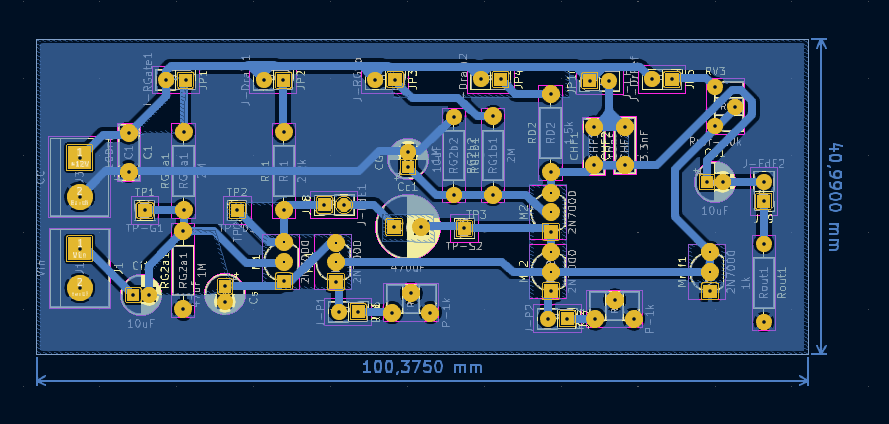
\includegraphics{Imagenes/Trazas.png}
  }
  \caption{Vista del Bottom Copper del diseño}
  \label{fig:trazas}
\end{figure}

\vspace{0.5em}
{\small\textbf{Diseño de Impresión }}

A continuación se presenta el diseño (\ref{fig:impreso}) utilizado para transferir las pistas a la placa de cobre

\begin{figure}[H]
  \centering
  \resizebox{250}{!}
  {
    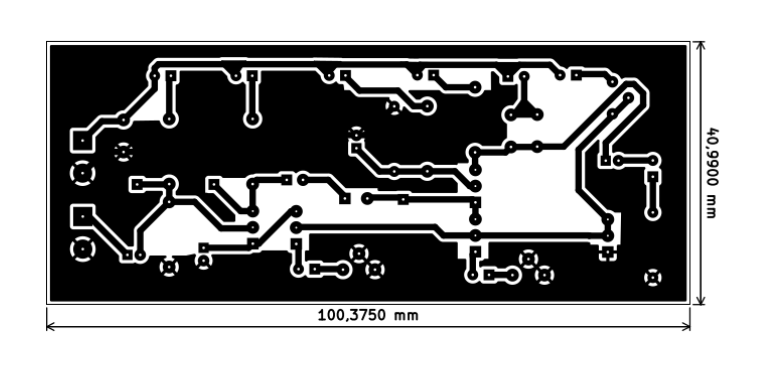
\includegraphics{Imagenes/Impreso.png}
  }
  \caption{Diseño de Impresión final}
  \label{fig:impreso}
\end{figure}
